\subsection{Die Datenbank}

Das in unserem System verwendete Datenbank-Management-System ist Postgres. Es läuft in einem eigenen Docker-Container. Da jede unserer Modellklassen weitere Funktionalität benötigt, haben wir eine abstrakte Modell-Klasse (\texttt{BaseModel}) definiert, welche als Superklasse für jede weitere Modellklasse dient, und welche selbst von \texttt{peewee.Model} erbt, wie in Abbildung \ref{fig:database-class} zu erkennen ist. Diese Funktionalitäten sind 
\begin{itemize}
	\item die expilizite Definition eines Primärschlüssels (\texttt{id}) mit dem Typ einer Zeichenkette, welcher einen Universally unique identifier (UUID) enthält,
	\item Daten, wann ein Objekt erzeugt und wann es zuletzt aktualisiert wurde
	\item und einen menschenlesbaren Bezeichner (\texttt{readable\_id}), welcher prozedural erzeugt wird und einer verbesserten Nutzerinteraktion dient.
\end{itemize}
Weiterhin wurde die Methode \texttt{save} überschrieben aus \texttt{peewee.Model} überschrieben, um darin den Feldern \texttt{created\_at}, \texttt{updated\_at} und \texttt{readable\_id} ihre Werte zuzuweisen.

\begin{figure}[!hb]
	\centering
	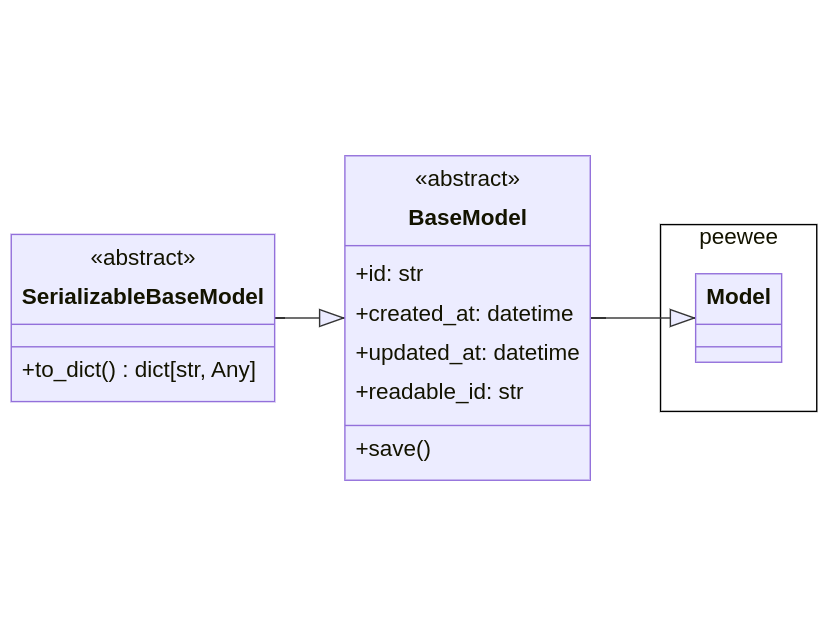
\includegraphics[width=0.75\linewidth]{images/diagrams/database-class.png}
	\caption{Klassendiagramm der abstrakten Modell-Klassen des ORM. \texttt{BaseModel} erbt von \texttt{peewee.Model}, um weitere Funktionalität hinzuzufügen. Davon erbt \texttt{SerializableBaseModel}, um die Serialisierung von Objekten zu ermöglichen.}
	\label{fig:database-class}
\end{figure}

Von \texttt{BaseModel} erbt \texttt{SerializableBaseModel}, welches die zusätzliche Methode \texttt{to\_dict} implementiert. Damit lässt sich das Objekt JSON-serialisieren, um es bei Bedarf an das Forntend der Anwendung senden zu können.

% \begin{figure}[!hb]
\begin{figure}[H]
	\centering
	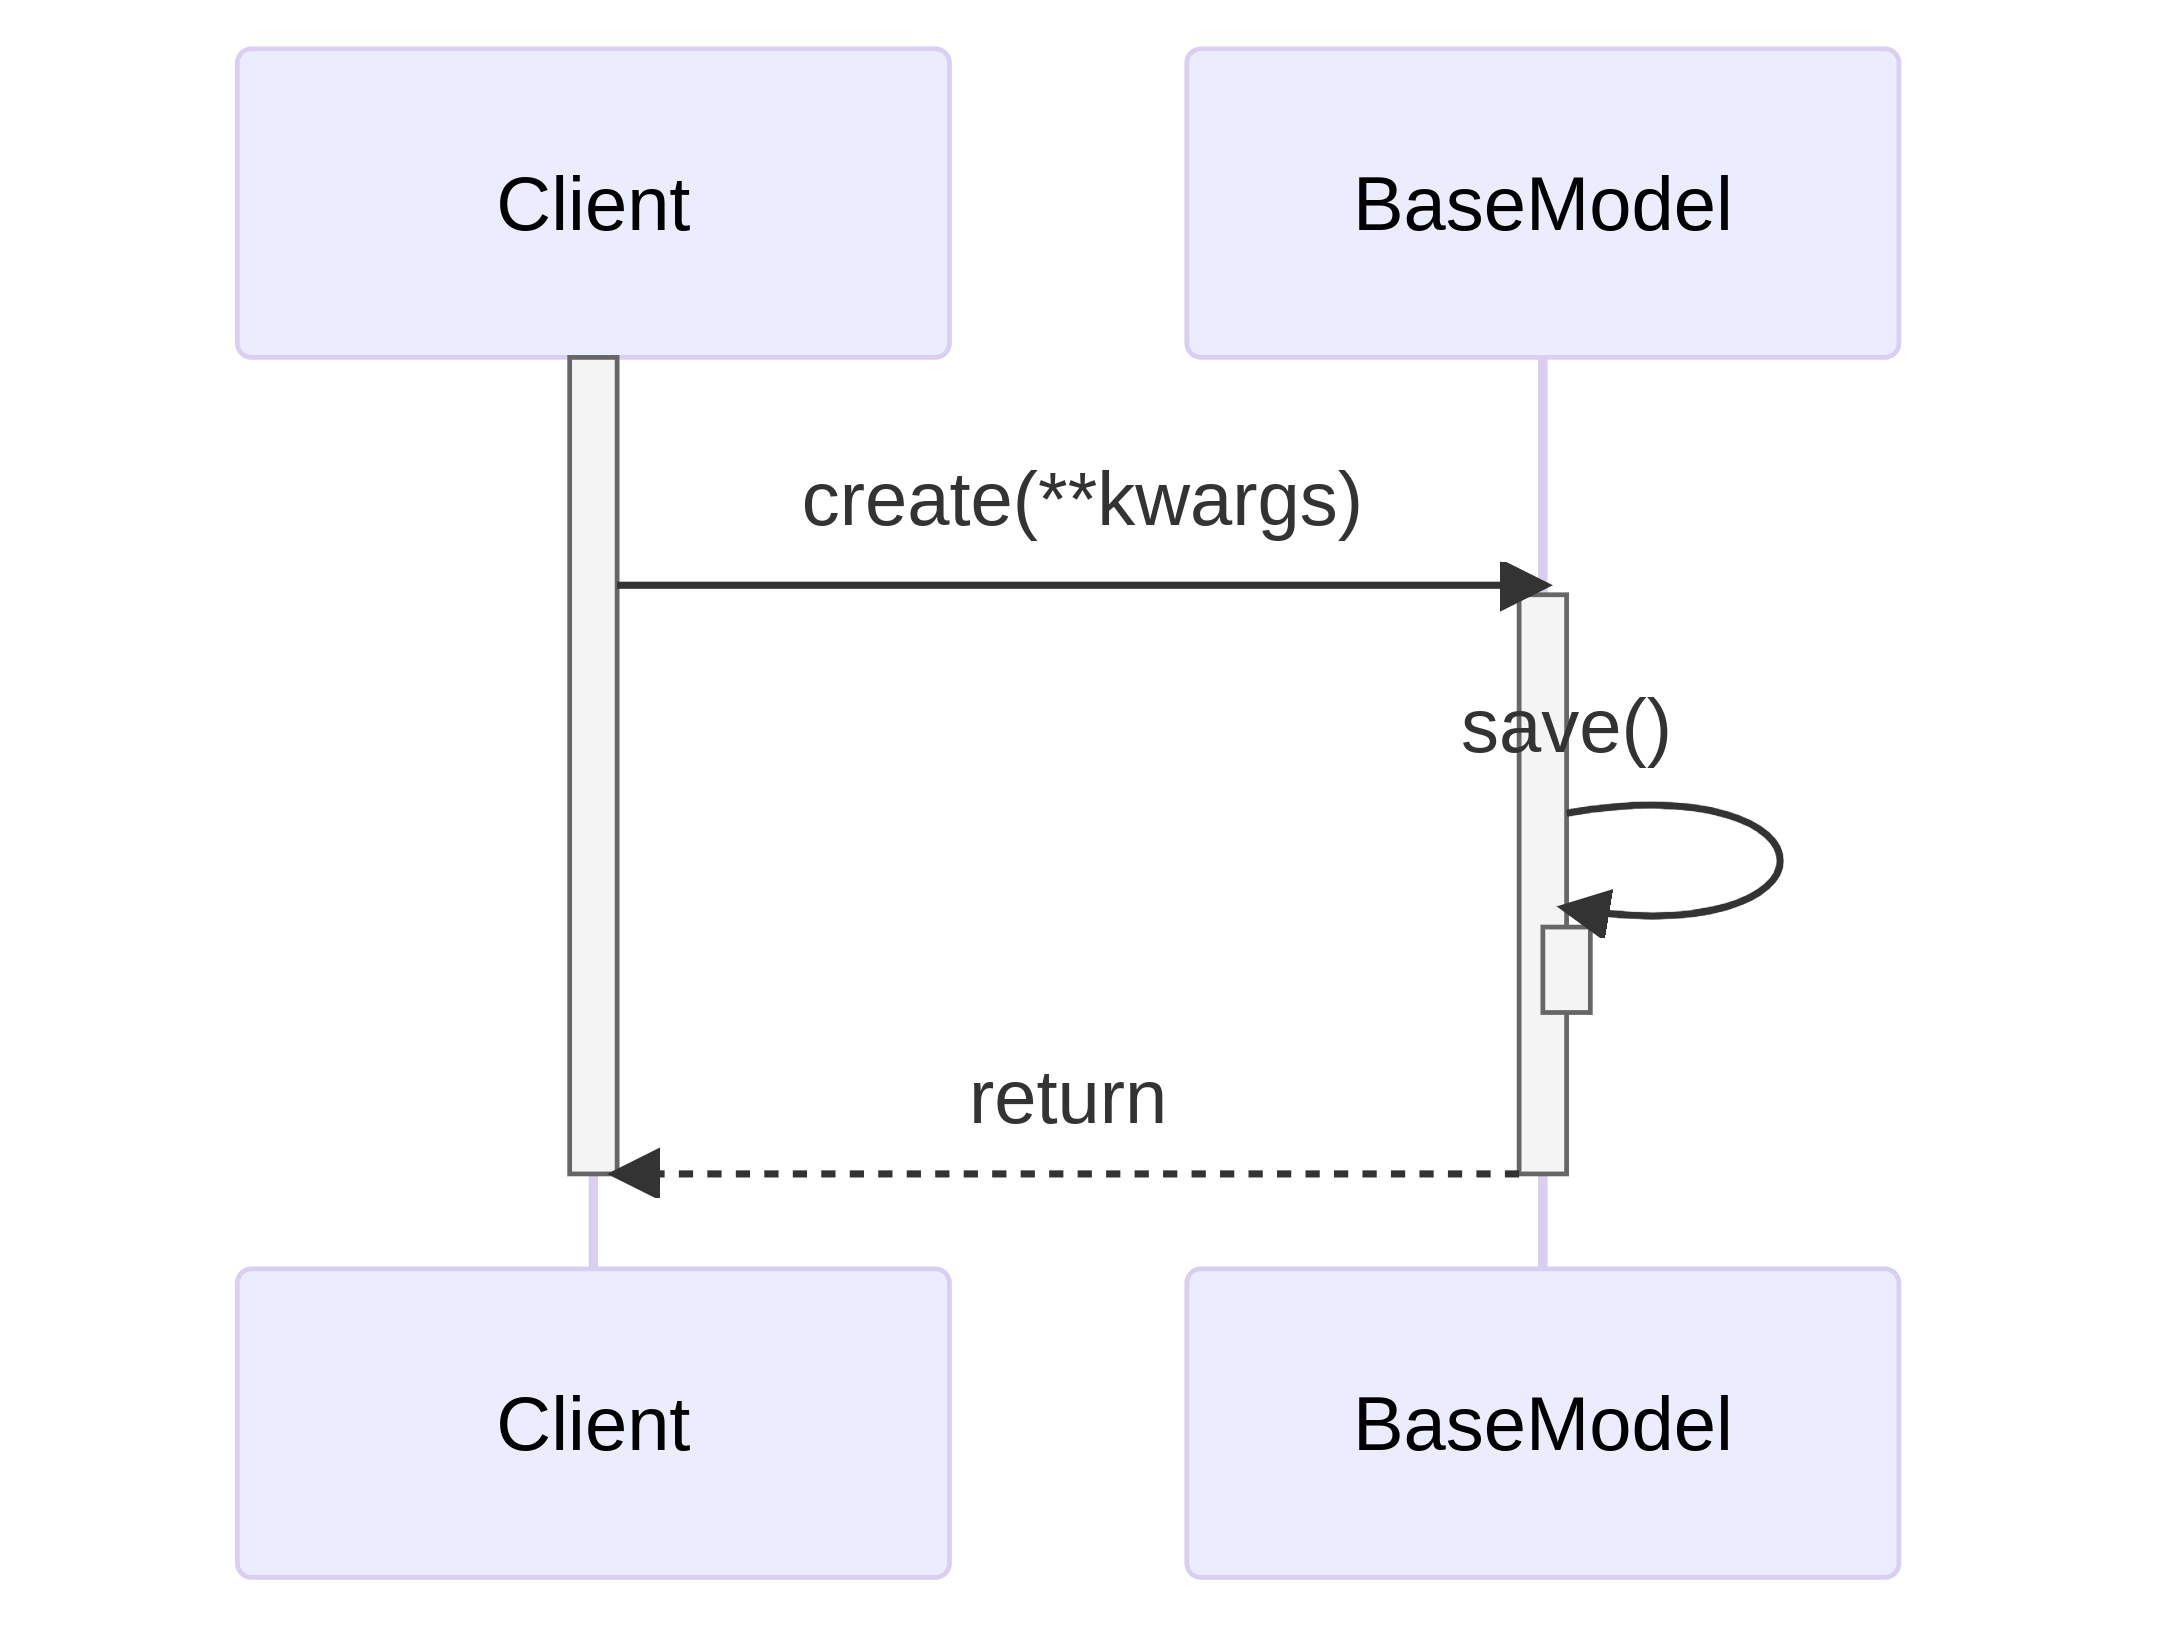
\includegraphics[width=0.75\linewidth]{images/diagrams/database-seq.png}
	\caption{Sequenzdiagramm der Erstellung eines Objektes über die Methode \texttt{create}.}
	\label{fig:database-seq}
\end{figure}

Da die hinzugefügten Funkionalitäten in der überschriebenen Methode \texttt{save} implementiert wurden, sind diese gut in das Modell-System von peewee integriert. Da \texttt{save} auch in \texttt{create} aufgerufen wird, wie in Abbildung \ref{fig:database-seq} zu erkennen, ist die Funktionalität damit automatisch auch bei der direkten Erzeugung eines neuen Objekts gegeben.

Alle im Rahmen unseres Projektes definierten Modell-Klassen erben von \texttt{BaseModel} oder \texttt{SerializableBaseModel} und erhalten damit die hinzugefügten Attribute.